\begin{wrapfigure}{l}{0.1\textwidth}
	\vspace{-10pt}
	
\includegraphics[width=\linewidth]{images/ikony_rhythmbox.png}
\end{wrapfigure}

Rhythmbox jest podstawowym odtwarzaczem muzyki w systemie Ubuntu. Dwukrotne kliknięcie pliku dźwiękowego otwiera program i rozpoczyna odtwarzanie wybranego pliku audio. Próba otwarcia w menadżerze plików wielu plików dźwiękowych na raz uruchamia Rhythmboksa i ustawia wszystkie wybrane pliki w kolejce odtwarzania.

Rhythmbox korzysta z zainstalowanych w systemie kodeków. Jeżeli postępując zgodnie z tym przewodnikiem zainstalowałeś pakiet \textcolor{ubuntu_orange}{ubuntu-restricted-extras}, to Rhythmbox będzie w stanie odtworzyć każdy popularny format audio.
\begin{center}
	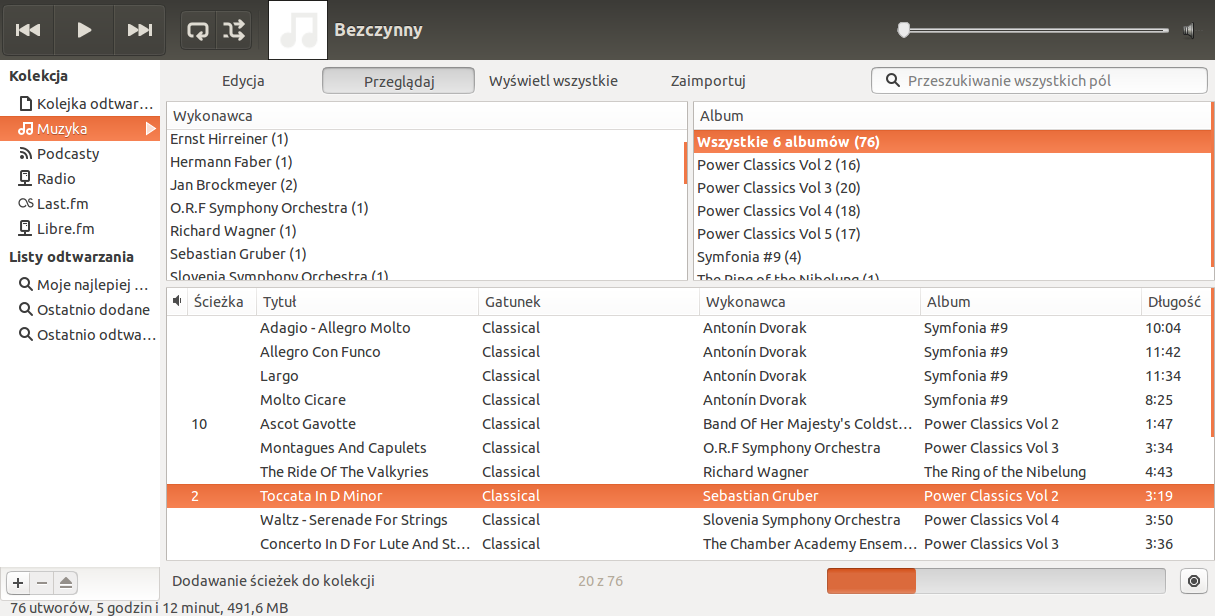
\includegraphics[width=\linewidth]{images/programy_rhythmbox1.png}
\end{center}
\clearpage
\subsubsection{Podstawy obsługi programu Rhythmbox}
\begin{wrapfigure}{r}{0.5\textwidth}
	\vspace{-10pt}
	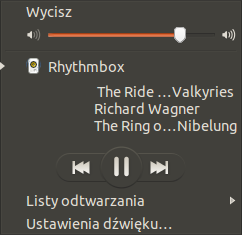
\includegraphics[width=\linewidth]{images/programy_rhythmbox2.png}
\end{wrapfigure}

Za pomocą systemowego menu ,,Dźwięk'' 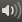
\includegraphics{images/ikony_dzwiek.png} możesz Rhythmboksa uruchomić, a następnie nim sterować (także innymi odtwarzaczami muzyki, jeżeli masz je zainstalowane). W tym menu wyświetlane są informacje o aktualnie odtwarzanym utworze oraz przyciski pozwalające kontrolować odtwarzacz muzyki, włączać listy odtwarzania, itp.

Kolekcja:
\begin{itemize}
\item Wszystkie pliki audio z katalogu Muzyka (który znajduje się w katalogu domowym) są automatycznie dodawane do kolekcji.
\item Aby wskazać inny katalog, wybierz \menu{{Modyfikuj}>{Preferencje}>{Muzyka}>{Pliki muzyczne znajdują się w:}} i wskaż który katalog program ma obserwować.
\item Wybierz \textcolor{ubuntu_orange}{Zaimportuj} w głównym oknie programu i wskaż katalog.
\end{itemize}
Odsłuchiwanie muzyki:
\begin{itemize}
\item Odtwarzanie rozpoczyna się po dwukrotnym kliknięciu pliku w głównym oknie programu. Po zakończeniu odtwarzania tego pliku Rhythmbox rozpocznie odtwarzanie kolejnego utworu z listy.
\item Zamknięcie okna programu nie powoduje przerwania odtwarzania. Rhythmbox może działać w~tle~---~wówczas można nim sterować za pośrednictwem ikony dźwięku 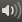
\includegraphics{images/ikony_dzwiek.png} na pasku menu.
\end{itemize}
Tworzenie kolejki odtwarzania:
\begin{enumerate}
\item Zaznacz jeden lub więcej utworów. Trzymając wciśnięty klawisz \keys{Shift} możesz zaznaczyć wiele kolejnych utworów. Trzymając wciśnięty klawisz \keys{CTRL} możesz kilknięciami myszy wybrać poszczególne utwory.
\item Kliknij i przytrzymaj wciśnięty lewy klawisz myszy, a następnie przesuń zaznaczone utwory na pozycję \textcolor{ubuntu_orange}{Kolejka odtwarzania}, znajdującą się w panelu po lewej.
\item Można również kliknąć prawym przyciskiem myszy i wybrać z menu kontekstowego \textcolor{ubuntu_orange}{Dodaj do kolejki}.
\end{enumerate}
Tworzenie listy odtwarzania:
\begin{enumerate}
\item Zaznacz jeden lub więcej utworów. Trzymając wciśnięty klawisz \keys{Shift} możesz zaznaczyć wiele kolejnych utworów. Trzymając wciśnięty klawisz \keys{CTRL} możesz kilknięciami myszy wybrać poszczególne utwory.
\item  Kliknij prawym przyciskiem myszy zaznaczone utwory i z menu kontekstowego wybierz \textcolor{ubuntu_orange}{Dodaj do listy odtwarzania}.
\begin{itemize}
\item \menu{{Dodaj no nowej listy odtwarzania}} utworzy nową listę odtwarzania. Pojawi się ona w panelu po lewej stronie okna. Klikając nową listę możesz zmienić jej nazwę.
\item Jeżeli masz już własne listy odtwarzania, to w tym menu możesz dodać do nich nowe utwory.
\end{itemize}
\end{enumerate}
